\begin{center}
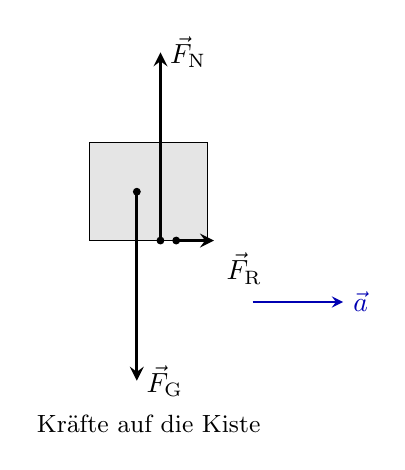
\begin{tikzpicture}[>=stealth]
 \draw[fill=gray!20] (-0.75,-0.62) rectangle (0.75,0.62);
 \draw[->, very thick] (-0.15,0) -- (-0.15,-2.4);
 \fill (-0.15,0) circle (0.05);
 \node[right] at (-0.15,-2.4) {$\vec F_\mathrm{G}$};
 \draw[->, very thick] (0.15,-0.62) -- (0.15,1.77);
 \fill (0.15,-0.62) circle (0.05);
 \node[right] at (0.15,1.77) {$\vec F_\mathrm{N}$};
 \draw[->, very thick] (0.35,-0.62) -- (0.83,-0.62);
 \fill (0.35,-0.62) circle (0.05);
 \node[below right=1pt] at (0.83,-0.62) {$\vec F_\mathrm{R}$};
 \draw[->, thick, blue!70!black] (1.32,-1.4) -- (2.47,-1.4) node[right] {$\vec a$};
 \node[font=\small] at (0,-2.95) {Kräfte auf die Kiste};
\end{tikzpicture}
\end{center}

\begin{abcliste}
\abc
Senkrecht heben sich Gewichtskraft und Normalkraft auf. Waagrecht wirkt nur eine Kraft auf die Kiste: die Haftreibung der Ladefläche. Sie ist also die resultierende Kraft und beschleunigt die Kiste:
\begin{align}
 \ssc{F}{R} &= \FRF \\
   &= \m\cdot\a \\
   &= \FR \approx \result{\FRP{0}{2}}
\end{align}
Die Haftreibung ist nur so gross wie nötig; $\mu_\mathrm{H}\,\ssc{F}{N}$ ist ihr grösstmöglicher Wert.

\abc
Die Haftreibung kann höchstens $\mu_\mathrm{H}\,\ssc{F}{N} = \mu_\mathrm{H}\,m\,g$ sein. Also
\begin{align}
 m\,\ssc{a}{max} &= \mu_\mathrm{H}\,m\,g \\
 \ssc{a}{max} &= \amaxF \\
   &= \muH\cdot\g \\
   &= \amax \approx \result{\amaxP{0}{2}}
\end{align}
Die Masse kürzt sich weg: Eine leichte Kiste rutscht genauso früh wie eine schwere.
\end{abcliste}
